

\chapter{Orbits}



%\section{Orbits}\label{2.1}
One crucial topic that anyone working with satellites needs to understand is orbits and their characteristics. An orbit is the \textbf{gravitationally curved path of an object around a center of mass}. Examples of orbits can be the Earth around the Sun or artificial satellites around the Earth.

This section will cover the elements that describe and define an orbit, how it is represented on a map and in which way the elements that define a particular orbit can be delivered so they can be used by a computer.


\section{Kepler's Laws}\label{2.1}
Planetary movements were first mathematically defined by the German mathematician, astronomer and astrologer Johannes Kepler in the 17th century. He concentrated his observations into three simple laws\citep{SSEng}:
\begin{itemize}

\item The orbit of each planet is an ellipse with the Sun occupying one focus.
\item The line joining the Sun to a planet sweeps out equal areas in equal intervals of time.
\item A planet's orbital period is proportional to the mean distance between the Sun and the planet, raised to the power of 3/2.
\end{itemize} 

These laws apply to every celestial body. When analysing to bodies, if one is much bigger than the other, it conforms the "two-body problem". It assumes that both bodies are spherical and they are modelled as if they were point particles. This means that influences from any third body are discarded. The analysis of hits problem has resulted in six elements that completely define an orbit, which will be explained in the next section.


\pagebreak
\section{Classical Orbital Elements}\label{2.2}
The Classical Orbital Elements are six and uniquely identify an orbit. They also can be used to predict future positions.\cite{IntAstr}

The first two elements, the orbit's size and shape are defined based on a 2D representation on an ellipse (Figure \ref{f2.1}).

\begin{figure}[H]
\centerline{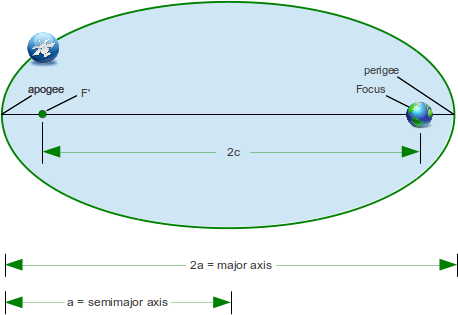
\includegraphics[width=0.7\textwidth]{images/Ellipse.png}}
\caption{Semimajor Axis}
\label{f2.1}
\end{figure}

\begin{itemize}
\item The \emph{semimajor axis} ($a$) is one half the distance across the long axis of the orbit, and it represents the orbit's size.
\item The \emph{eccentricity} represents the shape of the orbit. It describes how much the ellipse is elongated compared to a circle. Based on the latter, the orbit can have the following shapes, as shown in Figure \ref{f2.2}

\begin{figure}[H]
\centerline{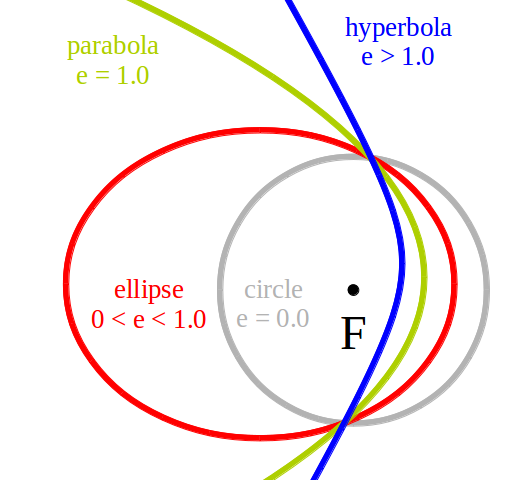
\includegraphics[scale=0.35]{images/Eccentricity.png}}
\caption{Eccentricity}
\label{f2.2}
\end{figure}

\end{itemize}


Before jumping onto the next Orbital E\section{Kepler's Laws}\label{2.1}lements it is necessary to point out that the Geocentric-equatorial Coordinate System will be used. It is now a 3D representation, where the fundamental plane is Earth's equatorial plane and the principal direction is in the vernal equinox direction.

The following orbital elements define the orientation of the orbital plane:

\begin{itemize}
\item The inclination ($i$) describes the tilt of the orbital plane with respect to the reference plane. It is measured at the ascending node. This is, where the orbit crosses with the reference plain when moving upwards.
\item The right ascension of the ascending node ($\Omega$) represents the angle between the principal direction and the point where the orbital plane crosses the reference plane from south to north measured eastward. 
\end{itemize}

Based on this two elements, the orbits can be classified as shown in Table \ref{Table2.1}

\begin{table}[h]
\centering
\begin{tabular}{|c|c|c|}
\hline
\begin{tabular}[x]{@{}c@{}}\textbf{Inclination ($i$)}\end{tabular} &
\begin{tabular}[x]{@{}c@{}}\textbf{Orbital Type}\end{tabular} &
\begin{tabular}[x]{@{}c@{}}\textbf{Diagram}\end{tabular}\\
\hline
\begin{tabular}[x]{@{}c@{}} 0$^\circ$ or 180$^\circ$\end{tabular} &
\begin{tabular}[x]{@{}c@{}}Equatorial\end{tabular} &
\begin{tabular}[x]{@{}c@{}}\raisebox{-\totalheight}{
\includegraphics[scale=0.5]{images/EquatorialOrbit.png}}\end{tabular}\\
\hline
\begin{tabular}[x]{@{}c@{}} 90$^\circ$\end{tabular} &
\begin{tabular}[x]{@{}c@{}}Polar\end{tabular} &
\begin{tabular}[x]{@{}c@{}}\raisebox{-\totalheight}{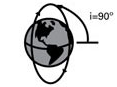
\includegraphics[scale=0.5]{images/PolarOrbit.png}}\end{tabular}\\
\hline
\begin{tabular}[x]{@{}c@{}} 0$^\circ$ $\leq$ $i$ $<$ 90$^\circ$\end{tabular} &
\begin{tabular}[x]{@{}c@{}}Direct or Prograde (moves in the\\ direction of Earth's rotation)\end{tabular} &
\begin{tabular}[x]{@{}c@{}}\raisebox{-\totalheight}{
\includegraphics[scale=0.5]{images/DirectOrbit.png}}\end{tabular}\\
\hline
\begin{tabular}[x]{@{}c@{}} 90$^\circ$ $<$ $i$ $\leq$ 180$^\circ$\end{tabular} &
\begin{tabular}[x]{@{}c@{}}Indirect or Retrograde (moves against\\ the direction of Earth's rotation)\end{tabular} &
\begin{tabular}[x]{@{}c@{}}\raisebox{-\totalheight}{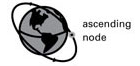
\includegraphics[scale=0.5]{images/IndirectOrbit.png}}\end{tabular}\\
\hline
\end{tabular}
 \caption{Types of Orbits and Their Inclination \cite{IntAstr}.}
  \label{Table2.1}
\end{table}


Although it is not part of the COEs, orbits can also be sorted by their altitude. NASA's classification divides orbits in three groups (Table \ref{Table2.2}).

\begin{table}[h]
\centering
\begin{tabular}{|c|c|c|}
\hline
\begin{tabular}[x]{@{}c@{}}\textbf{Orbit}\end{tabular} &
\begin{tabular}[x]{@{}c@{}}\textbf{Altitude ($a$)}\end{tabular} &
\begin{tabular}[x]{@{}c@{}}\textbf{Uses}\end{tabular}\\
\hline
\begin{tabular}[x]{@{}c@{}}Low Earth Orbit (LEO)\end{tabular} &
\begin{tabular}[x]{@{}c@{}}$a < 2000 Km$\end{tabular} &
\begin{tabular}[x]{@{}c@{}}Scientific and weather\\ satellites
\end{tabular}\\
\hline
\begin{tabular}[x]{@{}c@{}}Medium Earth Orbit (MEO)\end{tabular} &
\begin{tabular}[x]{@{}c@{}}$2000 Km \leq a < 36000 Km$\end{tabular} &
\begin{tabular}[x]{@{}c@{}}GPS\end{tabular}\\
\hline
\begin{tabular}[x]{@{}c@{}}High Earth Orbit (HEO) or \\
Geosynchronous (GSO)\end{tabular} &
\begin{tabular}[x]{@{}c@{}}$36000 Km$\end{tabular} &
\begin{tabular}[x]{@{}c@{}}Communications\\(phones, television,\\ radio)
\end{tabular}\\
\hline
\end{tabular}
 \caption{NASA's classification of orbits. \cite{NASAOrbits}}
  \label{Table2.2}
\end{table}
\pagebreak

It is now time to go through the last two COEs:
\begin{itemize}
\item The argument of perigee ($\omega$) is the angle between the ascending node and the perigee, measured in the direction of the satellite's motion.
\item The true anomaly ($\upsilon$) specifies the location of the satellite within the orbit. Amongst all the CEOs, this is te only one which changes over time. It is the angle between the perigee and the satellite's position vector measured in the direction of its motion.
\end{itemize}

\begin{figure}[H]
\centerline{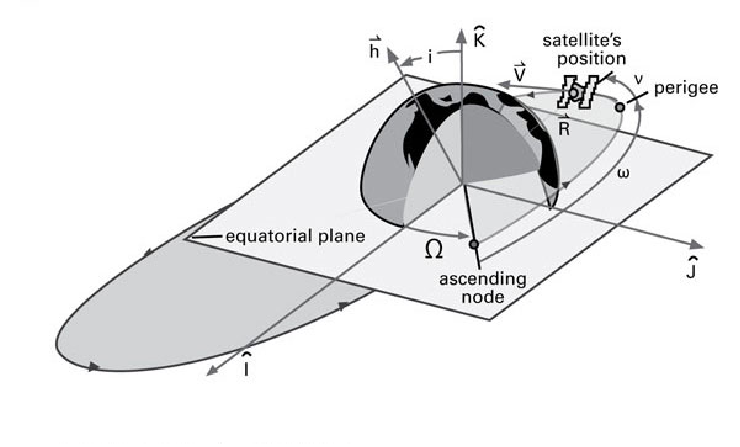
\includegraphics[width=0.7\textwidth]{images/COEs.png}}
\caption{Classical Orbital Elements \cite{IntAstr}}
\label{f2.3}
\end{figure}
\pagebreak
\section{Ground Tracks}\label{2.3}

The satellite ground tracks are the projection of its orbit onto Earth. An example of this can be Figure \ref{f2.4}.

\begin{figure}[H]
\centerline{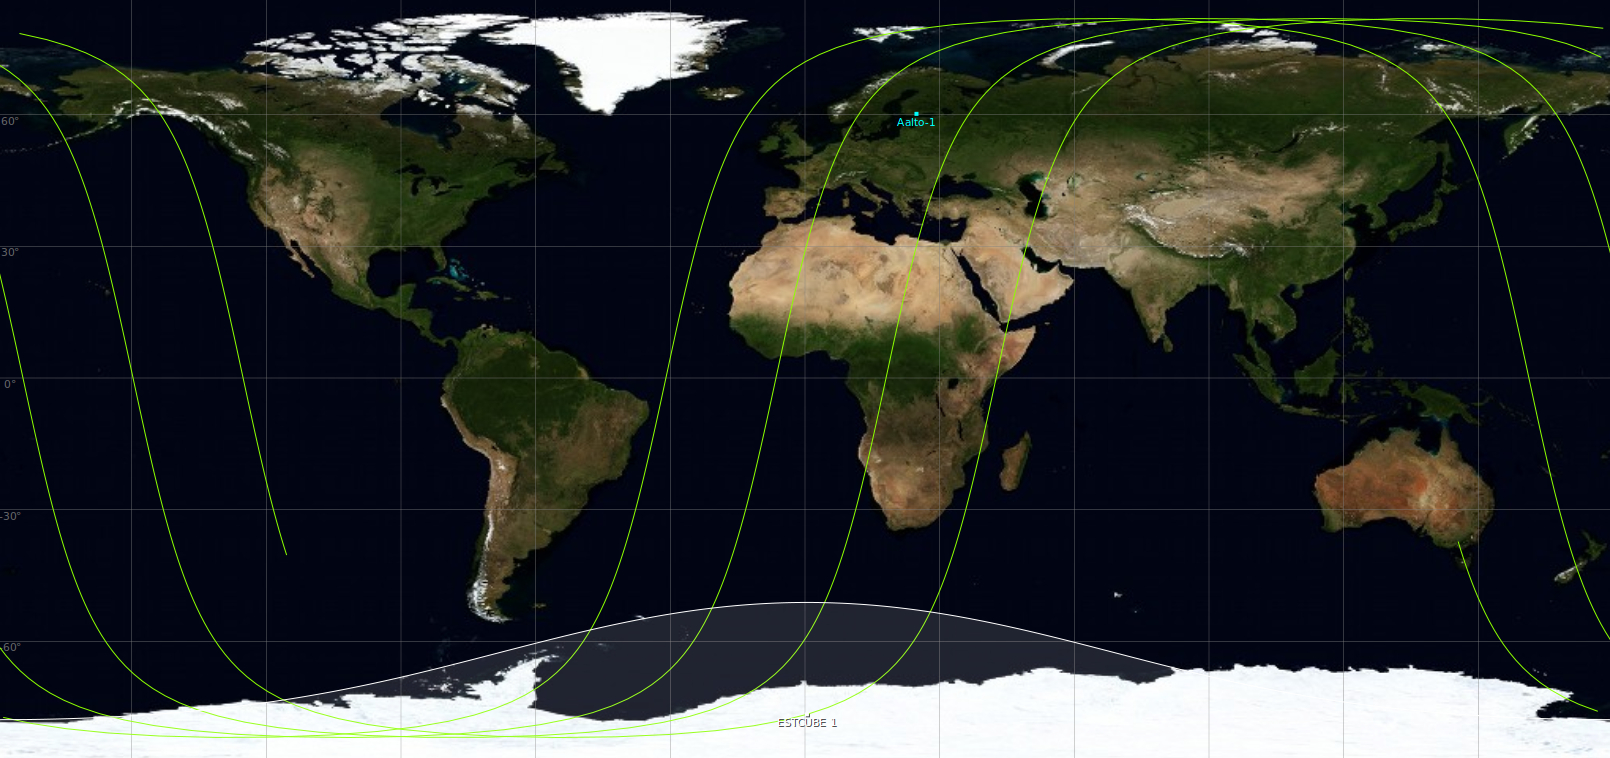
\includegraphics[width=1\textwidth]{images/GroundTracks.png}}
\caption{Ground Tracks of ESTCube-1}
\label{f2.4}
\end{figure}

Since the orbital plane does not move in inertial space, the satellite's orbit will always be the same. If Earth did not move the representation of the orbit would be a single line, as the ground track would continuously repeat. However, Earth rotates at 1600 km/hr. Thus, even if the orbit does not change, from the Earth-based observer's point of view it appears to shift to the west.

\section{Two Line Elements}\label{2.4}
A two line element set (TLE) is a data format created by the North American Aerospace Defense Command (NORAD) and NASA to transport sets of orbital elements describing satellite orbits around Earth. These TLEs can be later processed by a computer to calculate the position of a satellite at a particular time.
\newpage
The following snippet shows an example of a TLE for the International Space Station.

\noindent \texttt{\footnotesize ISS (ZARYA)\newline
1 25544U 98067A   13166.62319444  .00005748  00000-0  10556-3 0   120\newline
2 25544  51.6483 116.0964 0010829  73.3727 265.7013 15.50799671834453}\\

\begin{table}[h]
\centering
\begin{tabular}{|l|l|l|l|}
\hline
\begin{tabular}[x]{@{}c@{}}\textbf{Field}\end{tabular} &
\begin{tabular}[x]{@{}c@{}}\textbf{Columns}\end{tabular} &
\begin{tabular}[x]{@{}c@{}}\textbf{Content}\end{tabular} &
\begin{tabular}[x]{@{}c@{}}\textbf{Example}\end{tabular}\\
\hline
\begin{tabular}[x]{@{}c@{}}1\end{tabular} &
\begin{tabular}[x]{@{}c@{}}01\end{tabular} &
\begin{tabular}[x]{@{}c@{}}Line number\end{tabular} &
\begin{tabular}[x]{@{}c@{}}1\end{tabular}\\
\hline
\begin{tabular}[x]{@{}c@{}}2\end{tabular} &
\begin{tabular}[x]{@{}c@{}}03-07\end{tabular} &
\begin{tabular}[x]{@{}c@{}}Satellite number\end{tabular} &
\begin{tabular}[x]{@{}c@{}}25544\end{tabular}\\
\hline
\begin{tabular}[x]{@{}c@{}}3\end{tabular} &
\begin{tabular}[x]{@{}c@{}}08\end{tabular} &
\begin{tabular}[x]{@{}c@{}}Classification (U=Unclassified)\end{tabular} &
\begin{tabular}[x]{@{}c@{}}U\end{tabular}\\
\hline
\begin{tabular}[x]{@{}c@{}}4\end{tabular} &
\begin{tabular}[x]{@{}c@{}}10-11\end{tabular} &
\begin{tabular}[x]{@{}l@{}}International Designator\\(Last two digits of launch year)\end{tabular} &
\begin{tabular}[x]{@{}c@{}}98\end{tabular}\\
\hline
\begin{tabular}[x]{@{}c@{}}5\end{tabular} &
\begin{tabular}[x]{@{}c@{}}12-14\end{tabular} &
\begin{tabular}[x]{@{}l@{}}International Designator\\ (Launch number of the year)\end{tabular} &
\begin{tabular}[x]{@{}c@{}}067\end{tabular}\\
\hline
\begin{tabular}[x]{@{}c@{}}6\end{tabular} &
\begin{tabular}[x]{@{}c@{}}15-17\end{tabular} &
\begin{tabular}[x]{@{}c@{}}International Designator (Piece of the launch)\end{tabular} &
\begin{tabular}[x]{@{}c@{}}A\end{tabular}\\
\hline
\begin{tabular}[x]{@{}c@{}}7\end{tabular} &
\begin{tabular}[x]{@{}c@{}}19-20\end{tabular} &
\begin{tabular}[x]{@{}l@{}}Epoch Year (Last two digits of year)\end{tabular} &
\begin{tabular}[x]{@{}c@{}}08\end{tabular}\\
\hline
\begin{tabular}[x]{@{}c@{}}8\end{tabular} &
\begin{tabular}[x]{@{}c@{}}21-32\end{tabular} &
\begin{tabular}[x]{@{}l@{}}Epoch (Day of the year and fractional\\portion of the day)\end{tabular} &
\begin{tabular}[x]{@{}c@{}}264.51782528\end{tabular}\\
\hline
\begin{tabular}[x]{@{}c@{}}9\end{tabular} &
\begin{tabular}[x]{@{}c@{}}34-43\end{tabular} &
\begin{tabular}[x]{@{}c@{}}First Time Derivative of the Mean Motion\end{tabular} &
\begin{tabular}[x]{@{}c@{}}-0.00002182\end{tabular}\\
\hline
\begin{tabular}[x]{@{}c@{}}10\end{tabular} &
\begin{tabular}[x]{@{}c@{}}45-52\end{tabular} &
\begin{tabular}[x]{@{}l@{}}Second Time Derivative of Mean Motion\\(decimal point assumed)\end{tabular} &
\begin{tabular}[x]{@{}c@{}}00000-0\end{tabular}\\
\hline
\begin{tabular}[x]{@{}c@{}}11\end{tabular} &
\begin{tabular}[x]{@{}c@{}}54-61\end{tabular} &
\begin{tabular}[x]{@{}c@{}}BSTAR drag term (decimal point assumed)\end{tabular} &
\begin{tabular}[x]{@{}c@{}}-11606-4\end{tabular}\\
\hline
\begin{tabular}[x]{@{}c@{}}12\end{tabular} &
\begin{tabular}[x]{@{}c@{}}63\end{tabular} &
\begin{tabular}[x]{@{}c@{}}Ephemeris type\end{tabular} &
\begin{tabular}[x]{@{}c@{}}0\end{tabular}\\
\hline
\begin{tabular}[x]{@{}c@{}}13\end{tabular} &
\begin{tabular}[x]{@{}c@{}}65-68\end{tabular} &
\begin{tabular}[x]{@{}c@{}}Element number\end{tabular} &
\begin{tabular}[x]{@{}c@{}}292\end{tabular}\\
\hline
\begin{tabular}[x]{@{}c@{}}14\end{tabular} &
\begin{tabular}[x]{@{}c@{}}69\end{tabular} &
\begin{tabular}[x]{@{}l@{}}Checksum (Modulo 10)\\(Letters, blanks, periods, plus signs = 0;\\minus signs = 1)\end{tabular} &
\begin{tabular}[x]{@{}c@{}}7\end{tabular}\\
\hline
\end{tabular}
 \caption{Two-Line Element Set Format Definition, Line 1} 
  \label{Table2.3}
\end{table}


\begin{table}
\centering
\begin{tabular}{|l|l|l|l|}
\hline
\begin{tabular}[x]{@{}c@{}}\textbf{Field}\end{tabular} &
\begin{tabular}[x]{@{}c@{}}\textbf{Columns}\end{tabular} &
\begin{tabular}[x]{@{}c@{}}\textbf{Content}\end{tabular} &
\begin{tabular}[x]{@{}c@{}}\textbf{Example}\end{tabular}\\
\hline
\begin{tabular}[x]{@{}c@{}}1\end{tabular} &
\begin{tabular}[x]{@{}c@{}}01\end{tabular} &
\begin{tabular}[x]{@{}c@{}}Line number\end{tabular} &
\begin{tabular}[x]{@{}c@{}}1\end{tabular}\\
\hline
\begin{tabular}[x]{@{}c@{}}2\end{tabular} &
\begin{tabular}[x]{@{}c@{}}03-07\end{tabular} &
\begin{tabular}[x]{@{}c@{}}Satellite number\end{tabular} &
\begin{tabular}[x]{@{}c@{}}25544\end{tabular}\\
\hline
\begin{tabular}[x]{@{}c@{}}3\end{tabular} &
\begin{tabular}[x]{@{}c@{}}09-16\end{tabular} &
\begin{tabular}[x]{@{}c@{}}Inclination [Degrees]\end{tabular} &
\begin{tabular}[x]{@{}c@{}}51.6416\end{tabular}\\
\hline
\begin{tabular}[x]{@{}c@{}}4\end{tabular} &
\begin{tabular}[x]{@{}c@{}}18-25\end{tabular} &
\begin{tabular}[x]{@{}l@{}}Right Ascension of the Ascending\\Node [Degrees]\end{tabular} &
\begin{tabular}[x]{@{}c@{}}247.4627\end{tabular}\\
\hline
\begin{tabular}[x]{@{}c@{}}5\end{tabular} &
\begin{tabular}[x]{@{}c@{}}27-33\end{tabular} &
\begin{tabular}[x]{@{}l@{}}Eccentricity (decimal point assumed)\\ (Launch number of the year)\end{tabular} &
\begin{tabular}[x]{@{}c@{}}0006703\end{tabular}\\
\hline
\begin{tabular}[x]{@{}c@{}}6\end{tabular} &
\begin{tabular}[x]{@{}c@{}}35-42\end{tabular} &
\begin{tabular}[x]{@{}c@{}}Argument of Perigee [Degrees]\end{tabular} &
\begin{tabular}[x]{@{}c@{}}130.5360\end{tabular}\\
\hline
\begin{tabular}[x]{@{}c@{}}7\end{tabular} &
\begin{tabular}[x]{@{}c@{}}44-51\end{tabular} &
\begin{tabular}[x]{@{}l@{}}Mean Anomaly [Degrees]\end{tabular} &
\begin{tabular}[x]{@{}c@{}}325.0288\end{tabular}\\
\hline
\begin{tabular}[x]{@{}c@{}}8\end{tabular} &
\begin{tabular}[x]{@{}c@{}}53-63\end{tabular} &
\begin{tabular}[x]{@{}l@{}}Mean Motion [Revs per day]\end{tabular} &
\begin{tabular}[x]{@{}c@{}}15.72125391\end{tabular}\\
\hline
\begin{tabular}[x]{@{}c@{}}9\end{tabular} &
\begin{tabular}[x]{@{}c@{}}64-68\end{tabular} &
\begin{tabular}[x]{@{}c@{}}Revolution number at epoch [Revs]\end{tabular} &
\begin{tabular}[x]{@{}c@{}}56353\end{tabular}\\
\hline
\begin{tabular}[x]{@{}c@{}}10\end{tabular} &
\begin{tabular}[x]{@{}c@{}}69\end{tabular} &
\begin{tabular}[x]{@{}l@{}}Checksum (Modulo 10)\end{tabular} &
\begin{tabular}[x]{@{}c@{}}00000-0\end{tabular}\\
\hline
\end{tabular}
 \caption{Two-Line Element Set Format Definition, Line 2} 
  \label{Table2.4}
\end{table}
